
%% bare_conf.tex
%% V1.3
%% 2007/01/11
%% by Michael Shell
%% See:
%% http://www.michaelshell.org/
%% for current contact information.
%%
%% This is a skeleton file demonstrating the use of IEEEtran.cls
%% (requires IEEEtran.cls version 1.7 or later) with an IEEE conference paper.
%%
%% Support sites:
%% http://www.michaelshell.org/tex/ieeetran/
%% http://www.ctan.org/tex-archive/macros/latex/contrib/IEEEtran/
%% and
%% http://www.ieee.org/

%%*************************************************************************
%% Legal Notice:
%% This code is offered as-is without any warranty either expressed or
%% implied; without even the implied warranty of MERCHANTABILITY or
%% FITNESS FOR A PARTICULAR PURPOSE! 
%% User assumes all risk.
%% In no event shall IEEE or any contributor to this code be liable for
%% any damages or losses, including, but not limited to, incidental,
%% consequential, or any other damages, resulting from the use or misuse
%% of any information contained here.
%%
%% All comments are the opinions of their respective authors and are not
%% necessarily endorsed by the IEEE.
%%
%% This work is distributed under the LaTeX Project Public License (LPPL)
%% ( http://www.latex-project.org/ ) version 1.3, and may be freely used,
%% distributed and modified. A copy of the LPPL, version 1.3, is included
%% in the base LaTeX documentation of all distributions of LaTeX released
%% 2003/12/01 or later.
%% Retain all contribution notices and credits.
%% ** Modified files should be clearly indicated as such, including  **
%% ** renaming them and changing author support contact information. **
%%
%% File list of work: IEEEtran.cls, IEEEtran_HOWTO.pdf, bare_adv.tex,
%%                    bare_conf.tex, bare_jrnl.tex, bare_jrnl_compsoc.tex
%%*************************************************************************

% *** Authors should verify (and, if needed, correct) their LaTeX system  ***
% *** with the testflow diagnostic prior to trusting their LaTeX platform ***
% *** with production work. IEEE's font choices can trigger bugs that do  ***
% *** not appear when using other class files.                            ***
% The testflow support page is at:
% http://www.michaelshell.org/tex/testflow/



% Note that the a4paper option is mainly intended so that authors in
% countries using A4 can easily print to A4 and see how their papers will
% look in print - the typesetting of the document will not typically be
% affected with changes in paper size (but the bottom and side margins will).
% Use the testflow package mentioned above to verify correct handling of
% both paper sizes by the user's LaTeX system.
%
% Also note that the "draftcls" or "draftclsnofoot", not "draft", option
% should be used if it is desired that the figures are to be displayed in
% draft mode.
%
\documentclass[conference]{IEEEtran}
\usepackage{blindtext, graphicx}

% Add the compsoc option for Computer Society conferences.
%
% If IEEEtran.cls has not been installed into the LaTeX system files,
% manually specify the path to it like:
% \documentclass[conference]{../sty/IEEEtran}





% Some very useful LaTeX packages include:
% (uncomment the ones you want to load)


% *** MISC UTILITY PACKAGES ***
%
%\usepackage{ifpdf}
% Heiko Oberdiek's ifpdf.sty is very useful if you need conditional
% compilation based on whether the output is pdf or dvi.
% usage:
% \ifpdf
%   % pdf code
% \else
%   % dvi code
% \fi
% The latest version of ifpdf.sty can be obtained from:
% http://www.ctan.org/tex-archive/macros/latex/contrib/oberdiek/
% Also, note that IEEEtran.cls V1.7 and later provides a builtin
% \ifCLASSINFOpdf conditional that works the same way.
% When switching from latex to pdflatex and vice-versa, the compiler may
% have to be run twice to clear warning/error messages.






% *** CITATION PACKAGES ***
%
\usepackage{cuted}
\usepackage{caption}
\usepackage{cite}
% cite.sty was written by Donald Arseneau
% V1.6 and later of IEEEtran pre-defines the format of the cite.sty package
% \cite{} output to follow that of IEEE. Loading the cite package will
% result in citation numbers being automatically sorted and properly
% "compressed/ranged". e.g., [1], [9], [2], [7], [5], [6] without using
% cite.sty will become [1], [2], [5]--[7], [9] using cite.sty. cite.sty's
% \cite will automatically add leading space, if needed. Use cite.sty's
% noadjust option (cite.sty V3.8 and later) if you want to turn this off.
% cite.sty is already installed on most LaTeX systems. Be sure and use
% version 4.0 (2003-05-27) and later if using hyperref.sty. cite.sty does
% not currently provide for hyperlinked citations.
% The latest version can be obtained at:
% http://www.ctan.org/tex-archive/macros/latex/contrib/cite/
% The documentation is contained in the cite.sty file itself.


\usepackage[cmex10]{amsmath}
\usepackage[algoruled,boxed,lined]{algorithm2e}
\usepackage{array}

\usepackage{lipsum}

\usepackage{mdwmath}
\usepackage{mdwtab}
% Also highly recommended is Mark Wooding's extremely powerful MDW tools,
% especially mdwmath.sty and mdwtab.sty which are used to format equations
% and tables, respectively. The MDWtools set is already installed on most
% LaTeX systems. The lastest version and documentation is available at:
% http://www.ctan.org/tex-archive/macros/latex/contrib/mdwtools/


% IEEEtran contains the IEEEeqnarray family of commands that can be used to
% generate multiline equations as well as matrices, tables, etc., of high
% quality.


\usepackage{eqparbox}
% Also of notable interest is Scott Pakin's eqparbox package for creating
% (automatically sized) equal width boxes - aka "natural width parboxes".
% Available at:
% http://www.ctan.org/tex-archive/macros/latex/contrib/eqparbox/





% *** SUBFIGURE PACKAGES ***
%\usepackage[tight,footnotesize]{subfigure}
% subfigure.sty was written by Steven Douglas Cochran. This package makes it
% easy to put subfigures in your figures. e.g., "Figure 1a and 1b". For IEEE
% work, it is a good idea to load it with the tight package option to reduce
% the amount of white space around the subfigures. subfigure.sty is already
% installed on most LaTeX systems. The latest version and documentation can
% be obtained at:
% http://www.ctan.org/tex-archive/obsolete/macros/latex/contrib/subfigure/
% subfigure.sty has been superceeded by subfig.sty.



%\usepackage[caption=false]{caption}
%\usepackage[font=footnotesize]{subfig}
% subfig.sty, also written by Steven Douglas Cochran, is the modern
% replacement for subfigure.sty. However, subfig.sty requires and
% automatically loads Axel Sommerfeldt's caption.sty which will override
% IEEEtran.cls handling of captions and this will result in nonIEEE style
% figure/table captions. To prevent this problem, be sure and preload
% caption.sty with its "caption=false" package option. This is will preserve
% IEEEtran.cls handing of captions. Version 1.3 (2005/06/28) and later 
% (recommended due to many improvements over 1.2) of subfig.sty supports
% the caption=false option directly:
%\usepackage[caption=false,font=footnotesize]{subfig}
%
% The latest version and documentation can be obtained at:
% http://www.ctan.org/tex-archive/macros/latex/contrib/subfig/
% The latest version and documentation of caption.sty can be obtained at:
% http://www.ctan.org/tex-archive/macros/latex/contrib/caption/




% *** FLOAT PACKAGES ***
%
\usepackage{fixltx2e}
% fixltx2e, the successor to the earlier fix2col.sty, was written by
% Frank Mittelbach and David Carlisle. This package corrects a few problems
% in the LaTeX2e kernel, the most notable of which is that in current
% LaTeX2e releases, the ordering of single and double column floats is not
% guaranteed to be preserved. Thus, an unpatched LaTeX2e can allow a
% single column figure to be placed prior to an earlier double column
% figure. The latest version and documentation can be found at:
% http://www.ctan.org/tex-archive/macros/latex/base/


\usepackage{tabularx,booktabs}
%\usepackage{stfloats}
% stfloats.sty was written by Sigitas Tolusis. This package gives LaTeX2e
% the ability to do double column floats at the bottom of the page as well
% as the top. (e.g., "\begin{figure*}[!b]" is not normally possible in
% LaTeX2e). It also provides a command:
%\fnbelowfloat
% to enable the placement of footnotes below bottom floats (the standard
% LaTeX2e kernel puts them above bottom floats). This is an invasive package
% which rewrites many portions of the LaTeX2e float routines. It may not work
% with other packages that modify the LaTeX2e float routines. The latest
% version and documentation can be obtained at:
% http://www.ctan.org/tex-archive/macros/latex/contrib/sttools/
% Documentation is contained in the stfloats.sty comments as well as in the
% presfull.pdf file. Do not use the stfloats baselinefloat ability as IEEE
% does not allow \baselineskip to stretch. Authors submitting work to the
% IEEE should note that IEEE rarely uses double column equations and
% that authors should try to avoid such use. Do not be tempted to use the
% cuted.sty or midfloat.sty packages (also by Sigitas Tolusis) as IEEE does
% not format its papers in such ways.





% *** PDF, URL AND HYPERLINK PACKAGES ***
%
\usepackage{url}
% url.sty was written by Donald Arseneau. It provides better support for
% handling and breaking URLs. url.sty is already installed on most LaTeX
% systems. The latest version can be obtained at:
% http://www.ctan.org/tex-archive/macros/latex/contrib/misc/
% Read the url.sty source comments for usage information. Basically,
% \url{my_url_here}.





% *** Do not adjust lengths that control margins, column widths, etc. ***
% *** Do not use packages that alter fonts (such as pslatex).         ***
% There should be no need to do such things with IEEEtran.cls V1.6 and later.
% (Unless specifically asked to do so by the journal or conference you plan
% to submit to, of course. )


% correct bad hyphenation here
\hyphenation{op-tical net-works semi-conduc-tor}

\ifCLASSOPTIONcompsoc
    \usepackage[caption=false, font=normalsize, labelfont=sf, textfont=sf]{subfig}
\else
\usepackage[caption=false, font=footnotesize]{subfig}
\fi


\begin{document}
%
% paper title
% can use linebreaks \\ within to get better formatting as desired
\title{An Approach for Multi Label Image Classification
Using Single Label Convolutional Neural Network
Classifier and Image Segmentation with Objectness Measure and Selective
Search}


% author names and affiliations
% use a multiple column layout for up to three different
% affiliations
%\author{\IEEEauthorblockN{Dr. Kazi Md. Rokibul Alam}
%\IEEEauthorblockA{Department of Computer Science and Engineering\\
%Khulna University of Engineering \& Technology\\
%Khulna, Bangladesh\\
%Email: rokibcse@yahoo.com}
%\and
%\IEEEauthorblockN{Setu Basak}
%\IEEEauthorblockA{Department of Computer Science and Engineering\\
%Khulna University of Engineering \& Technology\\
%Khulna, Bangladesh\\
%Email: setu.1421@yahoo.com}
%\and
%\centering
%\IEEEauthorblockN{Shubhashis Karmakar}
%\IEEEauthorblockA{Department of Computer Science and Engineering\\
%Khulna University of Engineering \& Technology\\
%Khulna, Bangladesh\\
%Email: shubhashis@gmail.com}
%\and
%
%}


\author{\IEEEauthorblockN{Dr. Kazi Md. Rokibul Alam\IEEEauthorrefmark{1},
Setu Basak\IEEEauthorrefmark{2}, Shubhashis Karmakar\IEEEauthorrefmark{3}}
\IEEEauthorblockA{Department of Computer Science and Engineering,
Khulna University of Engineering \& Technology\\
Khulna, Bangladesh\\
Email: \IEEEauthorrefmark{1}rokibcse@yahoo.com,
\IEEEauthorrefmark{2}setu.1421@yahoo.com,
\IEEEauthorrefmark{3}shubhashis@gmail.com}}

% conference papers do not typically use \thanks and this command
% is locked out in conference mode. If really needed, such as for
% the acknowledgment of grants, issue a \IEEEoverridecommandlockouts
% after \documentclass

% for over three affiliations, or if they all won't fit within the width
% of the page, use this alternative format:
% 
%\author{\IEEEauthorblockN{Michael Shell\IEEEauthorrefmark{1},
%Homer Simpson\IEEEauthorrefmark{2},
%James Kirk\IEEEauthorrefmark{3}, 
%Montgomery Scott\IEEEauthorrefmark{3} and
%Eldon Tyrell\IEEEauthorrefmark{4}}
%\IEEEauthorblockA{\IEEEauthorrefmark{1}School of Electrical and Computer Engineering\\
%Georgia Institute of Technology,
%Atlanta, Georgia 30332--0250\\ Email: see http://www.michaelshell.org/contact.html}
%\IEEEauthorblockA{\IEEEauthorrefmark{2}Twentieth Century Fox, Springfield, USA\\
%Email: homer@thesimpsons.com}
%\IEEEauthorblockA{\IEEEauthorrefmark{3}Starfleet Academy, San Francisco, California 96678-2391\\
%Telephone: (800) 555--1212, Fax: (888) 555--1212}
%\IEEEauthorblockA{\IEEEauthorrefmark{4}Tyrell Inc., 123 Replicant Street, Los Angeles, California 90210--4321}}




% use for special paper notices
%\IEEEspecialpapernotice{(Invited Paper)}




% make the title area
\maketitle


\begin{abstract}
%\boldmath
Single label image classification has been promisingly demonstrated using Convolutional Neural Network (CNN). However, how this CNN will fit for multi-label images is still difficult to solve. It is mainly difficult due to the complex underlying
object layouts and insufficient multi-label training images. This work has proposed an approach for classifying multi-label image by a trained single label classifier using CNN with objectness measure and selective search. We have taken two established image segmentation techniques for segmenting a single image which is a multi-label image into some segmented images. Then we have forwarded the images to our trained CNN and predicted the labels of the segmented images by generalizing the result. Our single-label image classifier gives 87\% accuracy on CIFAR-10 dataset. Using objectness measure with CNN gives us 51\% accuracy on a multi-label dataset and gives upto 57\% accuracy using selective search both considering top-4 labels which is significantly good for a simple approach rather than a complex approach of multi-label classifier using CNN.

\end{abstract}
% IEEEtran.cls defaults to using nonbold math in the Abstract.
% This preserves the distinction between vectors and scalars. However,
% if the journal you are submitting to favors bold math in the abstract,
% then you can use LaTeX's standard command \boldmath at the very start
% of the abstract to achieve this. Many IEEE journals frown on math
% in the abstract anyway.

% Note that keywords are not normally used for peerreview papers.
\begin{IEEEkeywords}
Image Classification, CNN, Objectness Measure, Selective Search.
\end{IEEEkeywords}






% For peer review papers, you can put extra information on the cover
% page as needed:
% \ifCLASSOPTIONpeerreview
% \begin{center} \bfseries EDICS Category: 3-BBND \end{center}
% \fi
%
% For peerreview papers, this IEEEtran command inserts a page break and
% creates the second title. It will be ignored for other modes.
\IEEEpeerreviewmaketitle



\section{Introduction}
In the computer vision field, there has been increasing interest in object category recognition. Among the major tasks, image classification is defined as the task of assigning an image one or multiple labels corresponding to the presence of a category in the image.\\
Multi-label image classification is however a more
general and practical problem, since the majority of real-world images are with more than one objects
of different categories. Many methods
have been proposed to address this more challenging
problem. The success of CNN on single-label image
classification also sheds some light on the multi-label image classification problem. However, the CNN
model cannot be trivially extended to cope with the
multi-label image classification problem in an interpretable manner, mainly due to the following reasons.
Firstly, the implicit assumption that foreground objects are roughly aligned, which is usually true for
single-label images, does not always hold for multi-label images. Such alignment facilitates the design of
the convolution and pooling infrastructure of CNN
for single-label image classification. However, for a
typical multi-label image, different categories of objects are located at various positions with different
scales and poses. For example, as shown in Figure \ref{fig1},
for single-label images, the foreground objects are
roughly aligned, while for multi-label images, even
with the same label, i.e., cat and bird, the spatial arrangements of the cat and bird instances
vary largely among different images. Secondly, the
interaction between different objects in multi-label
images, like partial visibility and occlusion, also poses
a great challenge. Therefore, directly applying the
original CNN structure for multi-label image classification is not feasible. Thirdly, due to the tremendous
parameters to be learned for CNN, a large number of
training images are required for the model training.
Furthermore, from single-label to multi-label (with n
category labels) image classification, the label space
has been expanded from n to 2n, thus more training data is required to cover the whole label space. For
single-label images, it is practically easy to collect
and annotate the images. However, the burden of
collection and annotation for a large scale multi-label
image dataset is generally extremely high.\\
So we propose a simple technique using our trained single-label classifier of CNN with the objectness measure \cite{1} and selective search \cite{2}. First we segment a multi-label image into some segments or image windows using the two approaches and then test these images against our trained single label model and predict the multiple labels of the image. We have taken different approaches like taking top-1, top-2, total sum of the scores and cumulative percentage sum of the scores to predict the labels.

\begin{figure} 
    \centering
  \subfloat[a]{%
       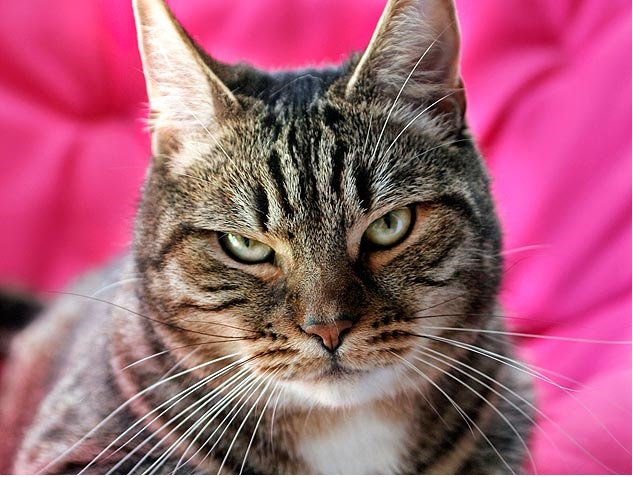
\includegraphics[width=0.2\linewidth]{images/1a}}
    \label{1a}
  \subfloat[b]{%
        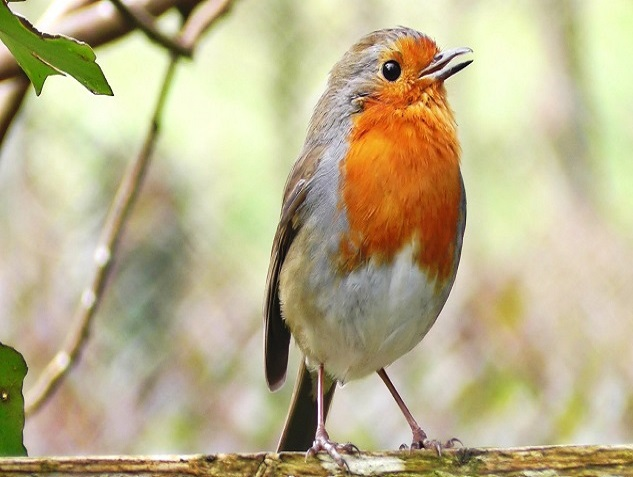
\includegraphics[width=0.2\linewidth]{images/1b}}
    \label{1b}
  \subfloat[c]{%
        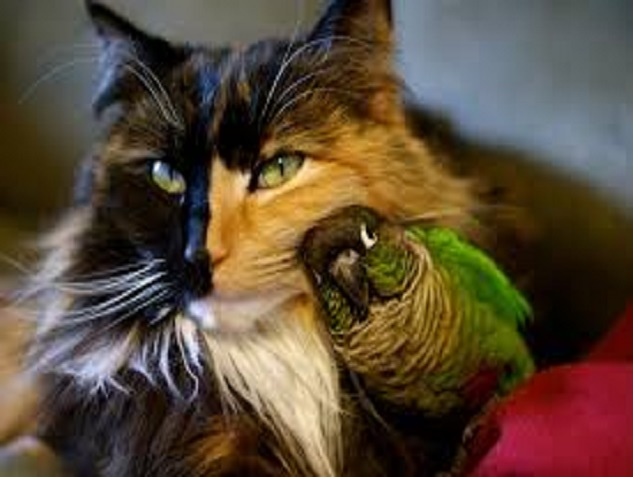
\includegraphics[width=0.2\linewidth]{images/1c}}
    \label{1c}
  \subfloat[d]{%
        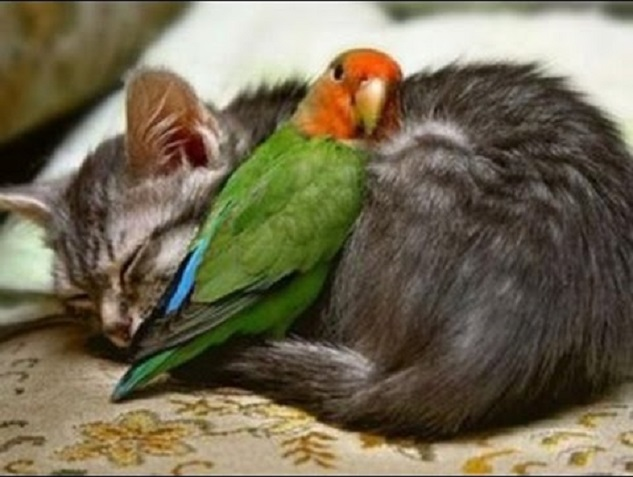
\includegraphics[width=0.2\linewidth]{images/1d}}
     \label{1d} 
  \caption{(a), (b) Some examples from CIFAR-10 \cite{4}. The objects in     
        single-label images are usually roughly aligned.(c),(d) However, the 
        assumption of object alignment is not valid for multi-label
        images. Also note the partial visibility and occlusion
        between objects in the multi-label images.}
        \vspace{-.5cm}
  \label{fig1} 
\end{figure}



%\newcolumntype{C}{>{\centering\arraybackslash}X} % centered version of "X" type
%\setlength{\extrarowheight}{1pt} % filler text
%\begin{table*}
% \caption{CIFAR-10 Confusion Matrix}
%\label{my-label}
%\begin{tabularx}{\textwidth}{@{}l*{10}{C}c@{}}
%\toprule
%labels     & airplane & automobile & bird & cat & deer & dog & frog & horse & ship & truck & accuracy \\ 
%\midrule
%airplane   & 915      & 4          & 17   & 19  & 3    & 1   & 0    & 2     & 27   & 12    & 91.50\%  \\ 
%automobile & 8        & 934        & 3    & 4   & 0    & 0   & 3    & 0     & 10   & 38    & 93.40\%  \\ 
%bird       & 60       & 1          & 813  & 37  & 19   & 23  & 30   & 10    & 7    & 0     & 81.30\%  \\ 
%cat        & 18       & 1          & 34   & 746 & 25   & 113 & 37   & 18    & 8    & 0     & 74.60\%  \\ 
%deer       & 24       & 1          & 38   & 33  & 809  & 19  & 44   & 29    & 2    & 1     & 80.90\%  \\ 
%dog        & 4        & 0          & 37   & 106 & 23   & 792 & 9    & 26    & 2    & 1     & 79.20\%  \\ 
%frog       & 2        & 5          & 19   & 35  & 1    & 20  & 912  & 2     & 3    & 1     & 91.20\%  \\ 
%horse      & 14       & 0          & 26   & 20  & 18   & 28  & 4    & 886   & 3    & 1     & 88.60\%  \\ 
%ship       & 35       & 10         & 3    & 2   & 0    & 2   & 1    & 0     & 936  & 11    & 93.60\%  \\ 
%truck      & 23       & 37         & 4    & 10  & 1    & 2   & 2    & 0     & 15   & 906   & 90.60\%  \\ 
%\bottomrule
%\end{tabularx}
%\end{table*}


\section{Related Works}
During the past few years, many works on various single-label and 
multi-label image classification models have been conducted. These models are generally based on deep learning.

\subsection{Deep Learning Based Models}

Deep learning tries to model the high-level abstractions of visual data by using architectures composed of multiple non-linear transformations. Specifically, deep convolutional neural network (CNN)
has demonstrated an extraordinary ability for image classification on single-label datasets such as CIFAR-10/100 \cite{4} and ImageNet \cite{3}. A. Krizhevsky et al. \cite{3}  trained one of the largest convolutional
neural networks to date on the subsets of ImageNet used in the ILSVRC-2010 and ILSVRC-2012
competitions. Their network contains
a number of new and unusual features which improve its performance. The size of their network made overfitting a significant problem, even
with 1.2 million labeled training examples, so they used several effective techniques for preventing
overfitting. Their final network contains five convolutional and
three fully-connected layers, and this depth seems to be important: they found that removing any
convolutional layer (each of which contains no more than 1\% of the model’s parameters) resulted in
inferior performance.\\
But their network is huge and complex. Their network’s size is limited mainly by the amount of memory available on current GPUs
and by the amount of training time that they are willing to tolerate. Their network takes between five
and six days to train on two GTX 580 3GB GPUs. All of their experiments suggest that their results
can be improved simply by waiting for faster GPUs and bigger datasets to become available.\\
More recently, CNN architectures have been
adopted to address multi-label problems. Gong et
al. \cite{5} studied and compared several multi-label
loss functions for the multi-label annotation problem
based on a similar network structure to \cite{3}.\\
However,
due to the large number of parameters to be learned
for CNN, an effective model requires lots of training
samples. Therefore, training a task-specific convolutional neural network is not applicable on datasets
with limited numbers of training samples.









\section{Dataset}
\subsection{CIFAR-10 Dataset}
The CIFAR-10 dataset is a subset of the 80 million tiny images. They were collected by Alex Krizhevsky, Vinod Nair, and Geoffrey Hinton.
The CIFAR-10 dataset consists of 60000 32x32 color images in 10 classes, with 6000 images per class. There are 50000 training images and 10000 test images.
The dataset is divided into five training batches and one test batch, each with 10000 images. The test batch contains exactly 1000 randomly-selected images from each class. The training batches contain the remaining images in random order, but some training batches may contain more images from one class than another. Between them, the training batches contain exactly 5000 images from each class. The sample from CIFAR-10 dataset is given in Figure \ref{cifar10}.

\begin{figure}[h!]
  \centering
  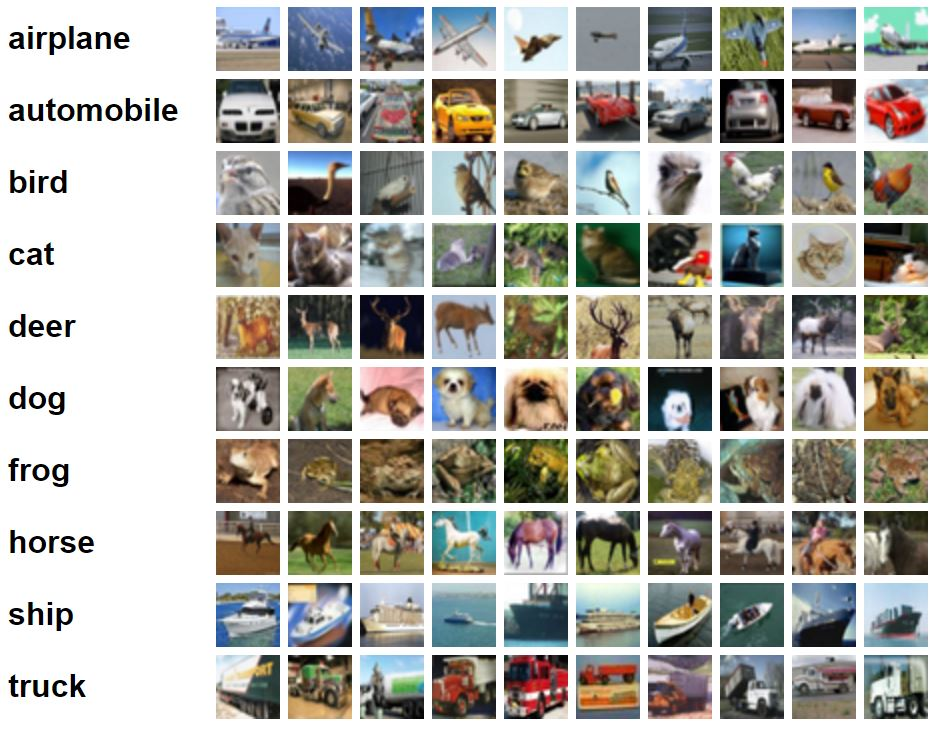
\includegraphics[width=.4\textwidth]{images/cifar10.JPG}
  \caption{CIFAR-10 Dataset} \label{cifar10}
  \vspace{-.5cm}
\end{figure}

\subsection{Multi Label Dataset}
As we are using single label dataset(CIFAR-10) for our single label Convolutional Neural Network, we have to use images that contain the identical contents from CIFAR-10. So, we picked random 100 images containing the identical contents as CIFAR-10 and tested it with our model. For an example, from Figure \ref{multi} we see that the image contains only a cat and a  dog, which our Single Label Convolutional Network can classify. So, the images we chose only contains subset of airplane, automobile, bird, cat, deer, dog, frog, horse, ship, truck.  

\begin{figure}[h!]
  \centering
  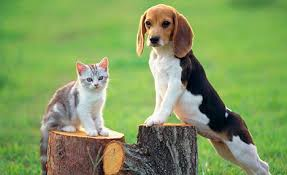
\includegraphics[width=.3\textwidth]{images/multi.jpg}
  \caption{Multi Label Image} \label{multi}
  \vspace{-.5cm}
\end{figure}

\section{Architecture}
\subsection{Architecture for classifying single label images}
Figure \ref{singlelabel} shows the Convolutional Neural Network that classifies single label images.In 
the each layer of Convolutional Neural Network from the Figure \ref{singlelabel}, the input image is converted by Spatial Convolution(number of input channels \(\rightarrow\) number of output channels, kernel height x kernel width, step height, step width, padding height, padding width). Then Spatial Batch Normalization is applied. After that Spatial Max Pooling(filter height, filter width, step height, step width) is used to downsample the images. Dropout is used to reduce overfitting. Rectifier Linear Unit is used for activation function. Also Linear Transformation(number of input channels \(\rightarrow\) number of output channels) is used to reduce the number of channels by applying linear transformation.

\begin{figure}[!htb]
  \centering
  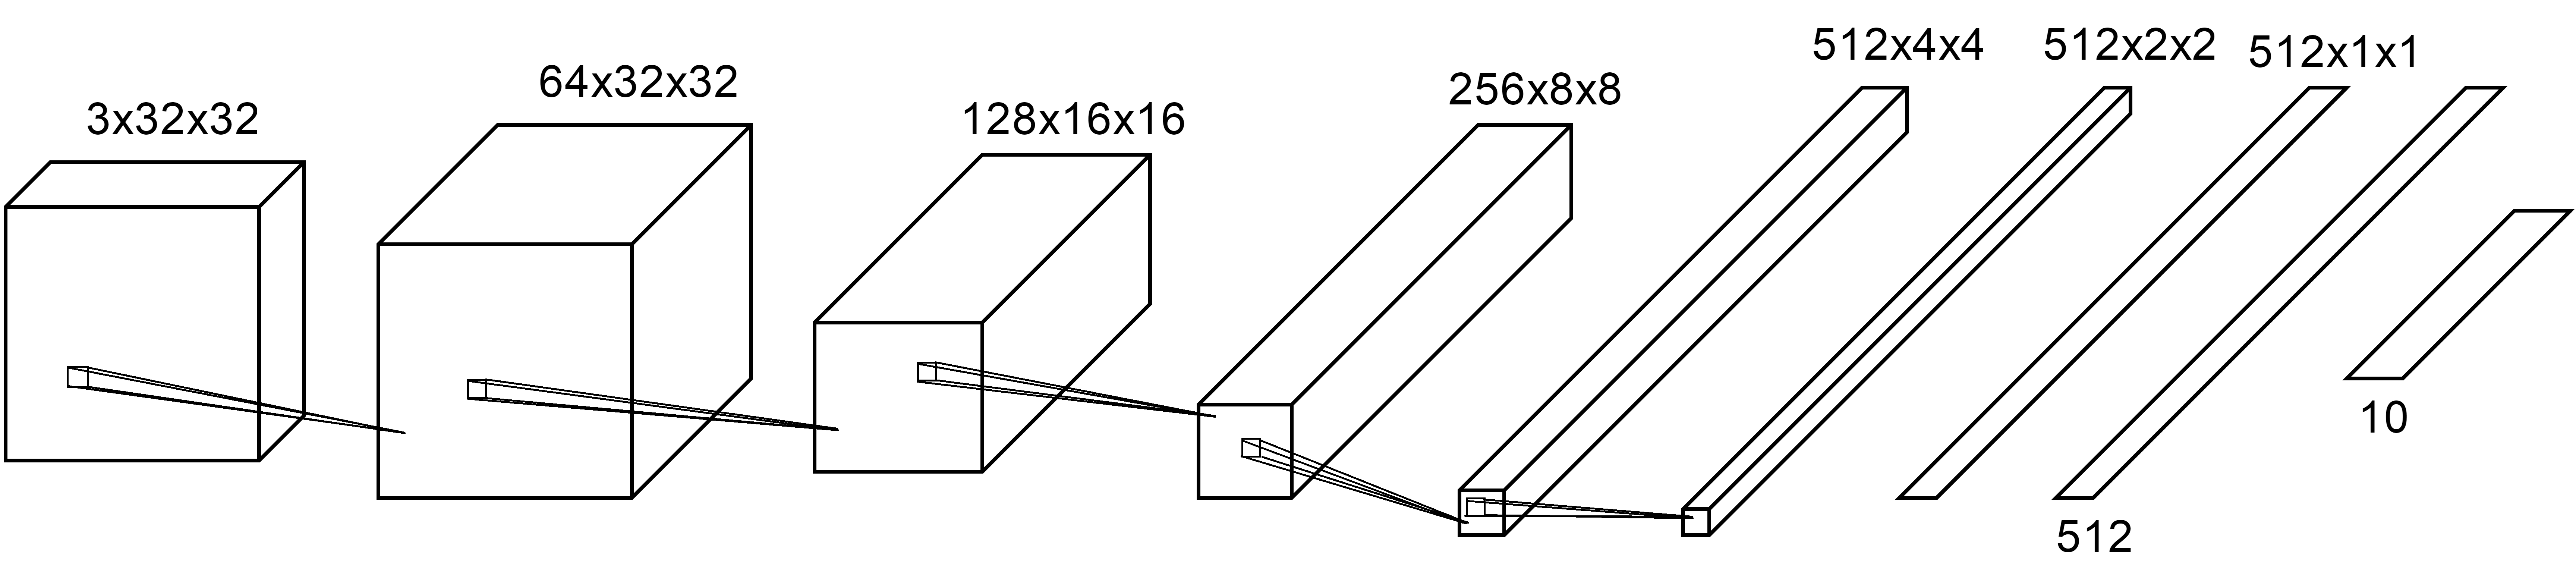
\includegraphics[width=.5\textwidth]{images/singlelabel.png}
  \caption{Convolutional Neural Network for Classifying Single Label Images(Cropped Down)}
   \vspace{-.5cm} \label{singlelabel}
\end{figure} 


 \paragraph{Spatial Convolution}
  
  Applies a 2D convolution over an input image composed of several input planes. For an example, Spatial Convolution(3 \(\rightarrow\) 64, 3x3, 1,1, 1,1) means that number of input channel is 3, and the number of output channel is 64. The kernel size is 3x3 and as there are 64 output channels, there will be 64 kernels, each having dimension 3x3. The step of the convolution is 1 step for height and width. The padding is 1 for height and width. Let's visualize this. In the figure \ref{spatialconv} the input neurons are the ones representing each pixel of an image, the kernel size or the filter size is 5x5. This filter would iterate over every single pixel and for each pixel look at the 5x5 neighborhood and produce corresponding images. As the number of output channel is 64, this will be done 64 times.
  
  \begin{figure}[h!]
  \centering
  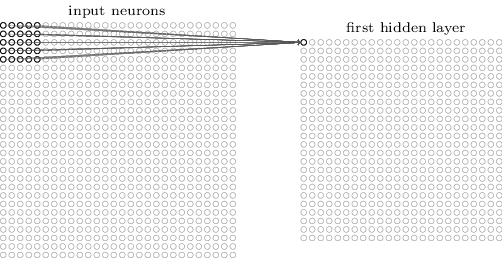
\includegraphics[width=.4\textwidth]{images/spatialconv.png}
  \caption{Spatial Convolution with Kernel Size 5x5} \label{spatialconv}
  \vspace{-.5cm}
\end{figure}

\paragraph{Spatial Batch Normalization}

Implements Batch Normalization as described in the paper FILL. The operation implemented is:

 $$y=\frac{x - mean(x)}{standard \textendash deviation(x)} * gamma + beta$$
 
 where the mean and standard-deviation are calculated per feature-map over the mini-batches and pixels and where gamma and beta are learnable parameter vectors of size N (where N = number of feature maps).
 
 
 \paragraph{ReLU}
 It is the activation function defined as: $$f(x) = max(0,x)$$.
 
 
 \paragraph{Spatial Max Pooling:}
 Applies 2D max-pooling operation. For example, Spatial Max Pooling(2,2,2,2) means that the max pooling will be done with filter 2x2 with step 2 in height and step 2 in width direction. Max pooling means that we will select the maximum value from 2x2 filter or the input area.
 
 
 \paragraph{Dropout}
 Dropout is used to prevent the neural network from overfitting. Dropout is implemented by only keeping a neuron active with some probability p (a hyperparameter), or setting it to zero otherwise. The input neuron is scaled by $1/p$ if it is not deactivated.
 
 \paragraph{Linear}
 Applies a linear transformation to the incoming data ($y = mx + c$). For example, Linear(512 \(\rightarrow\) 10) means that there are 512 input channels and these 512 channels are converted to 10 channels. So, the weight matrix will be 10x512. 
 
 
 \paragraph{Loss Function}
 Cross-entropy loss function has been used which has the form:
 
 
$$ L_{i} = -\log{(\frac{e^{f_y}}{\sum_j{e^{f_j}}})}$$

\paragraph{Normalization on CIFAR-10}

Normalization is required so that all the inputs are at a comparable range. This can be done to force the input values to a certain range. The images were converted from RGB channel to YUV channel. Then U and V channels were normalized globally with mean and standard deviation. The Y channel was normalized locally.

\subsection{Image Segmentation}
\subsubsection{Measuring the objectness of image windows}
B. Alexe et al. \cite{1} presented a generic objectness measure, quantifying how likely it is for an image window to contain an object of any
class. They explicitly trained it to distinguish objects with a well-defined boundary in space, such as cows and telephones, from amorphous
background elements, such as grass and road. The measure combines in a Bayesian framework several image cues measuring characteristics of objects, such as appearing
from their surroundings and having a closed boundary. These include an
innovative cue to measure the closed boundary characteristic. Finally, they presented two applications of objectness. In the first, they sample a small number windows according to their
objectness probability and gave an algorithm to employ them as location priors for modern class-specific object detectors. As they showed 
\begin{figure}[!htb]
    \centering
  \subfloat[a]{%
       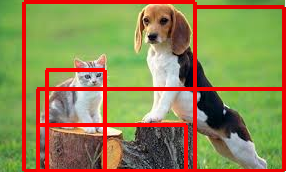
\includegraphics[width=0.4\linewidth]{images/obj1}}
    \label{obj1}
  \subfloat[b]{%
        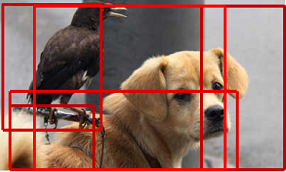
\includegraphics[width=0.4\linewidth]{images/obj2}}
    \label{obj2}
  \caption{Segmented Images}
        \vspace{-.5cm}
  \label{objectnessfig} 
\end{figure}
experimentally, this greatly reduces the number of windows evaluated by the expensive class-specific model. In the second application,
they used objectness as a complementary score in addition to the class-specific model, which leads to fewer false positives. As shown in
several recent papers, objectness can act as a valuable focus of attention mechanism in many other applications operating on image
windows, including weakly supervised learning of object categories, unsupervised pixelwise segmentation, and object tracking in video.
Computing objectness is very efficient and takes only about 4 sec. per image. This technique finds out some image windows like Figure \ref{objectnessfig}.\\
\begin{algorithm}
\SetAlgoLined
\centering
\begin{description}\itemsep0pt \parskip0pt \parsep0pt \vspace{.1cm}
  
  \item[Input:] \(F, D, c\) 
  \item[Ouput:] \(Det\)
  \item[Step 1:] \( \l = \left \{ w_{1},...,w_{F} \right \}, w_{i}\rightarrow D, \forall_{i} \)
  \item[Step 2:] \( \l_{s} = \left \{ \left ( w_{1},sw_{1} \right ),...,\left ( w_{F},sw_{F} \right )  \right \}, sw_{i}= c\left ( w_{i} \right ), \forall_{i} \) 
  \item[Step 3:] \( \rho _{s} = NMS\left ( \l_{s} \right )=\left \{ \left ( w_{n1},sw_{n1} \right ),...,\left ( w_{np},sw_{np} \right )  \right \}\)
  \item[Step 4:] \(\L=\left \{ w_{n1}^{lm},..., w_{np}^{lm} \right \}, w_{nj}^{lm} = max \left ( s_{w} \right )\)
  \item[Step 5:] \(Det = NMS\left ( \L \right )\)
\end{description}
\caption{Using objectness for class-specific detectors.}
\end{algorithm}
The general scheme for using their objectness measure as
a location prior for object detectors is algorithm 1. The
algorithm inputs the class-specific confidence function \(c\) which
the detector employs to score a window.
They build an initial set \(\l\) of \(F = 1000\) windows multinomially sampled from the distribution \(D\) of windows scored by
their objectness measure (Multi-scale Saliency)\(MS\) +(Color Contrast)\(CC\) + (Superpixels Straddling)\(SS\) (step 1). They use \(c\) to
score each window in \(\l\) (step 2). They then run the non-maxima
suppression. This results in a set \(\rho_{s}\) of promising
windows (step 3). For every window \(w_{p} \epsilon \rho_{s}\), they iteratively
move to the local maximum of \(c\) in its neighborhood \(V_{w
p}\),
resulting in window \(w_{p}^{lm}\) (step 4). Finally, they run \(NMS\) on the
local maxima windows \(\L\) and obtain detections \(Det\) (step 5).
In order to use this algorithm one has to specify a window
scoring function \(c\), which is specific to a particular detector
and object class, and a window neighborhood.

\subsubsection{Selective Search for Object Recognition}

J.R.R. Uijlings et al. \cite{2} took a hierarchical grouping algorithm to form the basis of their
selective search. Bottom-up grouping is a popular approach to segmentation, hence they adapted it for selective search. Because
the process of grouping itself is hierarchical, they can naturally generate locations at all scales by continuing the grouping process until
the whole image becomes a single region. This satisfies the condition of capturing all scales.
As regions can yield richer information than pixels, they wanted to
use region-based features whenever possible. To get a set of small
starting regions which ideally do not span multiple objects, they used the fast method of Felzenszwalb and Huttenlocher \cite{7}, which
found well-suited for such purpose.
Their grouping procedure now works as follows. They first used \cite{7}
to create initial regions. Then they used a greedy algorithm to iteratively group regions together: First the similarities between all
neighbouring regions are calculated. The two most similar regions
are grouped together, and new similarities are calculated between
the resulting region and its neighbours. The process of grouping
the most similar regions is repeated until the whole image becomes
a single region.


\subsection{Architecture For Classifying Multi-Label Images}

Our Final architecture for detecting multi-label images consists of (1) image segmentation and (2) convolutional neural network for detecting segmented images. The image segmentation techniques, objectness measures and selective search and the architecture for single label image detection has been described before. In the Figure \ref{finalarch} there is an overview of the architecture.

\begin{figure}[!htb]
  \centering
  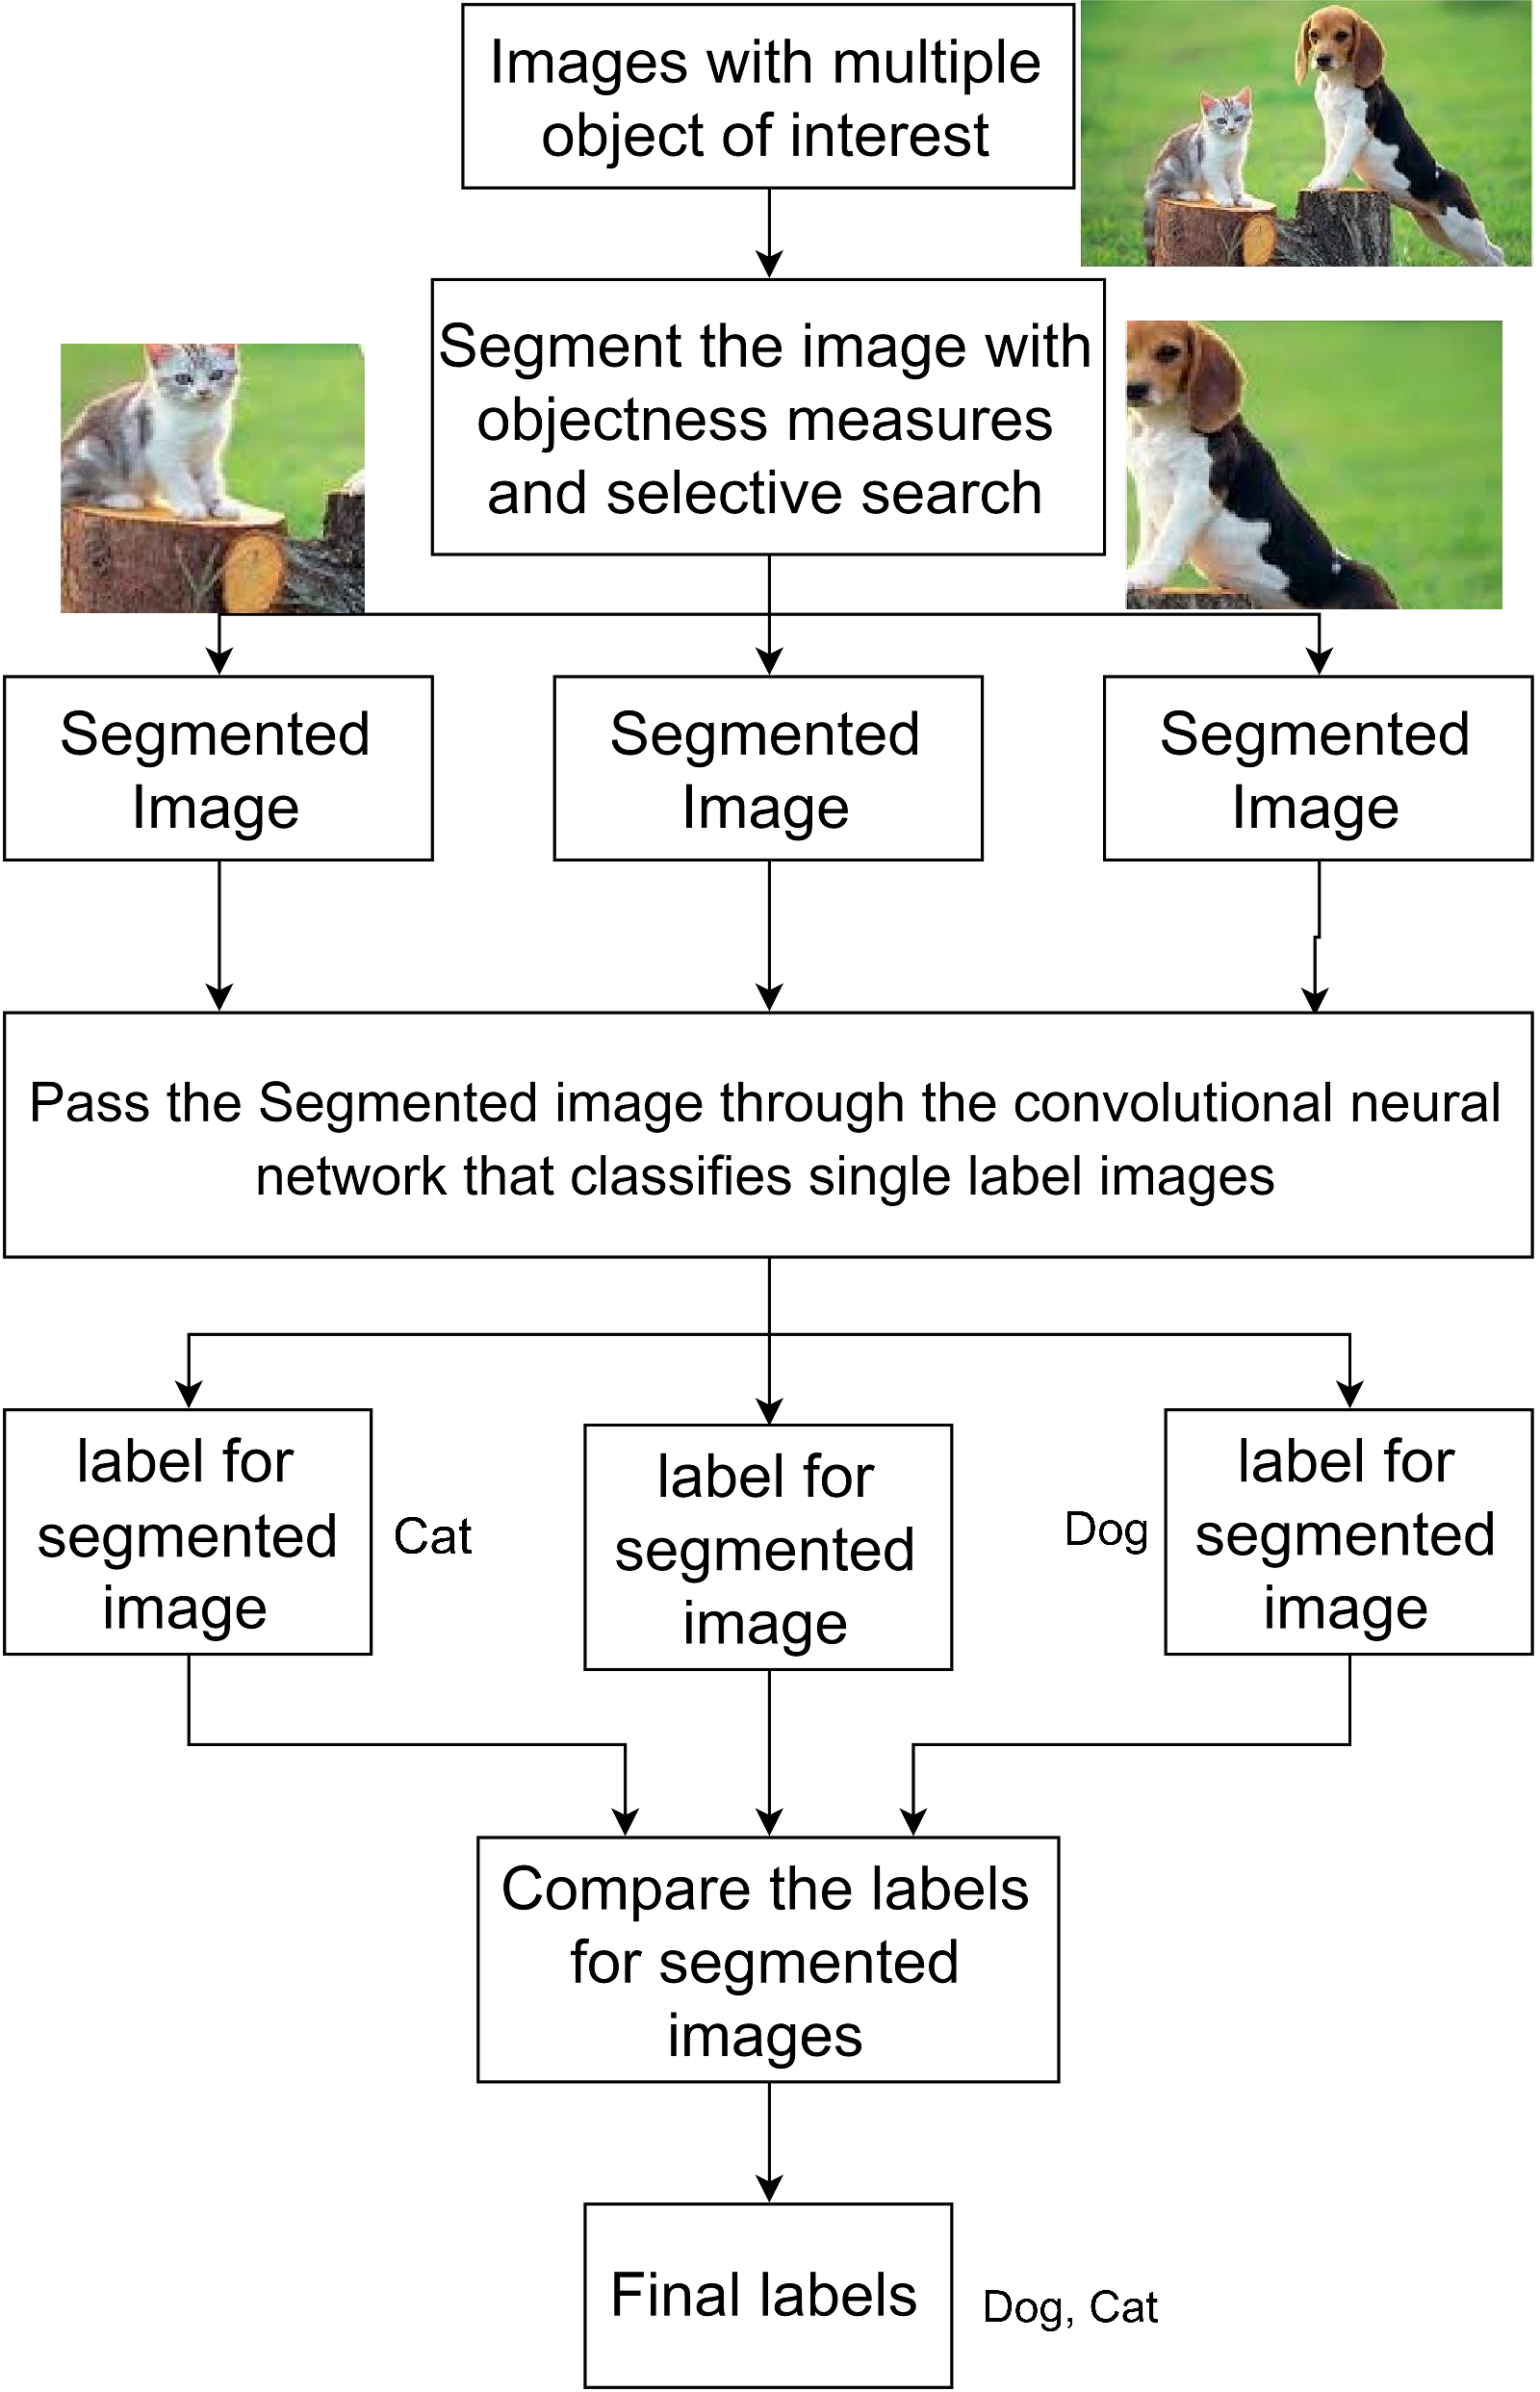
\includegraphics[width=0.4\textwidth]{images/finalarch.png}
  \caption{Architecture of Convolutional Neural Network}\label{finalarch}
\end{figure}

At first we split the image with objectness measures and selective search. Then we get multiple split images. Note that there will be many split images. In the figure only a few are shown. Then we pass the split images through the convolutional neural network that classifies the label associated with that image. As there are many split images, there may be some labels that will be wrongly classified. We inspect these labels and their associative scores and finally conclude which of the labels are likely to be associated with the images. We performed several techniques for inspecting the images. These are discussed in the experimental result section.


\section{Experimental Result}
\subsection{Experimental Result for CIFAR-10}

In the Table \ref{cifar10conf} there is the result for the testing images of CIFAR-10 dataset. Here, each row represents the testing label, each column represents the label produced by the network. For example the cell (1,1) represents that the testing label is airplane and the tagged label is airplane, the cell (1,2) represents that the testing label is airplane and the tagged label is automobile. So, each cell (i,i) where $[i = 1..10]$ represents the correctly tagged labels. Each row consists of 1000 image labels. So the accuracy will be cell$(i,i)/1000$.

%\begin{table}[!htb] 
% \centering
%  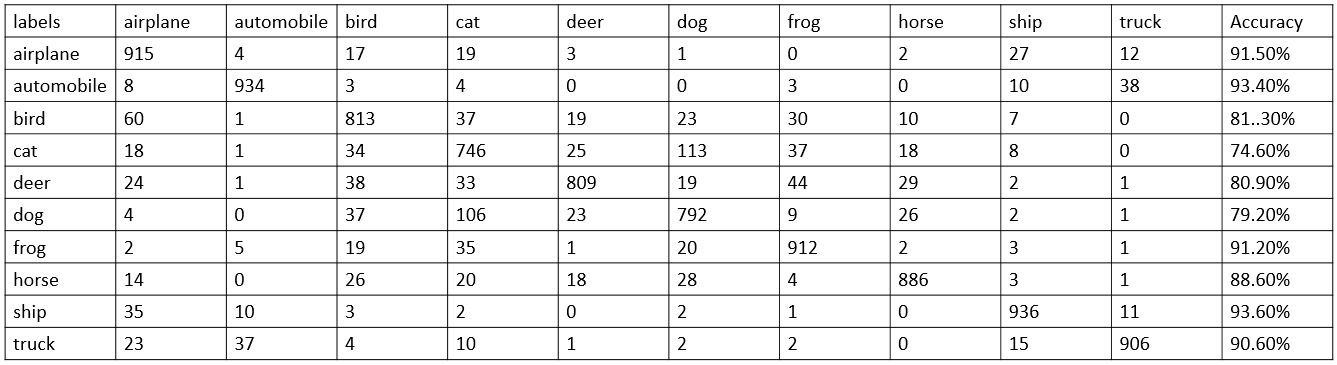
\includegraphics[width=0.9\textwidth]{images/cifar10.PNG}
%  \caption{CIFAR-10 Confusion Matrix}
%  \label{cifar10conf}
%\end{table}

\newcolumntype{C}{>{\centering\arraybackslash}X} % centered version of "X" type
\setlength{\extrarowheight}{1pt} % filler text
\begin{table*}
 \caption{CIFAR-10 Confusion Matrix}
\label{cifar10conf}
\begin{tabularx}{\textwidth}{@{}l*{10}{C}c@{}}
\toprule
labels     & airplane & automobile & bird & cat & deer & dog & frog & horse & ship & truck & accuracy \\ 
\midrule
airplane   & 915      & 4          & 17   & 19  & 3    & 1   & 0    & 2     & 27   & 12    & 91.50\%  \\ 
automobile & 8        & 934        & 3    & 4   & 0    & 0   & 3    & 0     & 10   & 38    & 93.40\%  \\ 
bird       & 60       & 1          & 813  & 37  & 19   & 23  & 30   & 10    & 7    & 0     & 81.30\%  \\ 
cat        & 18       & 1          & 34   & 746 & 25   & 113 & 37   & 18    & 8    & 0     & 74.60\%  \\ 
deer       & 24       & 1          & 38   & 33  & 809  & 19  & 44   & 29    & 2    & 1     & 80.90\%  \\ 
dog        & 4        & 0          & 37   & 106 & 23   & 792 & 9    & 26    & 2    & 1     & 79.20\%  \\ 
frog       & 2        & 5          & 19   & 35  & 1    & 20  & 912  & 2     & 3    & 1     & 91.20\%  \\ 
horse      & 14       & 0          & 26   & 20  & 18   & 28  & 4    & 886   & 3    & 1     & 88.60\%  \\ 
ship       & 35       & 10         & 3    & 2   & 0    & 2   & 1    & 0     & 936  & 11    & 93.60\%  \\ 
truck      & 23       & 37         & 4    & 10  & 1    & 2   & 2    & 0     & 15   & 906   & 90.60\%  \\ 
\bottomrule
\end{tabularx}
\end{table*}


\subsection{Experimental Result for Multi-Label Image tagging}
To give an overview of the process of inspecting the result of the segmented images, we will need the help of Table \ref{score}. The table is for a single multi-label image. Each $image_{i}$ represents the segmented image from the multi-label image. Each row represents the class scores given by the network. 

\paragraph{Selecting Top-1 Score:}
In this approach we select the top 1 score and its associating label from each segmented image $image_{i}$. Then we increase the frequency of labels for each top 1 score. After that we select the top 4 scoring labels. For example, in the Table \ref{score} the top 1 label for $image_{1}$ would be cat. So we increase the frequency of cat by 1. Similarly for $image_{2}$ again the score for label cat is highest. So frequency of cat will be increased by 1.

%\begin{table}[!htb]
% \centering
%  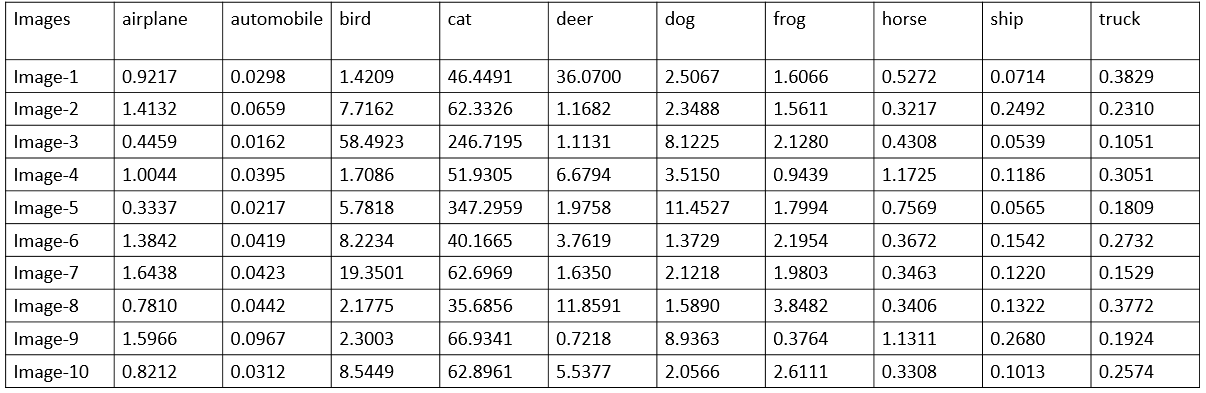
\includegraphics[width=0.9\textwidth]{images/newresult.PNG}
%  \caption{Scores for the sample image}
%  \label{score}
%\end{table}

\newcolumntype{C}{>{\centering\arraybackslash}X} % centered version of "X" type
\setlength{\extrarowheight}{1pt} % filler text
\begin{table*}
 \caption{Scores for the sample image}
\label{score}
\begin{tabularx}{\textwidth}{@{}l*{10}{C}c@{}}
\toprule
 Images    & airplane & automobile & bird & cat & deer & dog & frog & horse & ship & truck \\ 
\midrule
Image-1   & 0.9217  & 0.0298  & 1.4209  & 46.4491  & 36.0700 & 2.5067 & 1.6066  & 0.5272  & 0.0714   & 0.3829     \\ 
Image-2 & 1.4132  & 0.0659  & 7.7162  & 62.3326   & 1.1682     & 2.3488   & 1.5611    & 0.2317     & 0.2492 & 0.2310      \\ 
Image-3       & 0.4459       & 0.0162          & 58.4923  & 246.7195  & 1.1131   & 8.1225  & 2.1280   & 0.4308    & 0.0539    & 0.1051       \\ 
Image-4        & 1.0044       & 0.0395          & 1.7086   & 51.9305 & 6.6794   & 3.5150 & 0.9439   & 1.1725    & 0.1186    & 0.3051       \\ 
Image-5       & 0.3337       & 0.0217          & 5.7818   & 347.2959  & 1.9758  & 11.4527  & 1.7994   & 0.7569    & 0.0565    & 0.1809       \\ 
Image-6        & 1.3842        & 0.0419          & 8.2234   & 40.1665 & 3.7619   & 1.3729 & 2.1954    & 0.3672    & 0.1542    & 0.2732       \\ 
Image-7       & 1.6438        & 0.0423          & 19.3501   & 62.6969  & 1.6350    & 2.1218  & 1.9803  & 0.3463     & 0.1220    & 0.1529       \\ 
Image-8      & 0.7810       & 0.0442          & 2.1775   & 35.6856  & 11.8591   & 1.5890  & 3.8482    & 0.3406   & 0.1322    & 0.3772       \\ 
Image-9      & 1.5966       & 0.0967         & 2.3003    & 66.9341   & 0.7218    & 8.9363   & 0.3764    & 1.1311     & 0.2680  & 0.1924      \\ 
Image-10      & 0.8212       & 0.0312         & 8.5449    & 62.8961  & 5.5377    & 2.0566   & 2.6111    & 0.3208     & 0.1013   & 0.2574     \\ 
\bottomrule
\end{tabularx}
\end{table*}


\paragraph{Selecting Top-2 Score:}
In this approach we select the top 2 scores and its associating label from each segmented image $image_{i}$. Then we increase the frequency of labels for each top 2 scores. After that we select the top 4 scoring labels.  For example, in the Table \ref{score} the top 2 labels for $image_{1}$ would be cat and deer. So the frequency of cat and deer will be increased by 1.


%\begin{table}[!htb]
%\centering
%  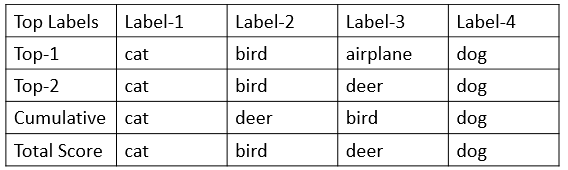
\includegraphics[width=0.9\textwidth]{images/result_objectness.PNG}
%  \caption{Result for the sample image for Objectness Measures}
%   \label{resobj}
%\end{table}

%\newcolumntype{C}{>{\centering\arraybackslash}X} % centered version of "X" type
%\setlength{\extrarowheight}{1pt} % filler text
%\begin{table*}
% \caption{Result for the sample image for Objectness Measures}
%\label{my-label}
%\begin{tabularx}{\textwidth}{@{}l*{10}{C}c@{}}
%\toprule
%Top Labels     & Label-1 & Label-2 & Label-3 & Label-4  \\ 
%\midrule
%Top-1          & cat      & bird         & airplane   & dog    \\ 
%Top-2          & cat      & bird         & deer       & dog    \\ 
%Cumulative     & cat      & deer         & bird       & dog    \\ 
%Total Score    & cat      & bird         & deer       & dog   \\ 
%\bottomrule
%\end{tabularx}
%\end{table*}

\begin{table}
\centering
\caption{Result for the sample image for Objectness Measures}
\label{resobj}
\begin{tabularx}{\linewidth}{|*{5}{X|}}
\hline
Labels      & Label-1 & Label-2 & Label-3 & Label-4 \\ \hline
Top-1       & cat     & bird   & airplane & dog           \\ \hline
Top-2       & cat     & bird   & deer     & dog           \\ \hline
Cumulative  & cat     & deer   & bird     & dog            \\ \hline
Total Score & cat     & bird   & deer     & dog           \\ \hline
\end{tabularx}
\end{table}
\paragraph{Selecting Total Score:}
In this approach we just add all scores of each $label_{i}$ for each segmented image $image_{i}$. Then we select the top 4 scoring labels. For example, every class score for every label will be added. So, the score for cat label will be the total score in the column cat. Similarly the score for bird will be the total score in the column bird.



\paragraph{Selecting Cumulative Percentage:}
Each $label_{i}$ of segmented image $image_{i}$ has the percentage $score_{i} / \sum_{i}{score_{i}}$. We select the top percentage from each segmented image $image_{i}$. We add these percentages for each associated labels and select the top 4 scoring labels. For example for $image_{1}$ the percentage of cat will be $score_{cat} / \sum_{i}{score_{i}}$.\hfill \break

The results for these four approaches for the sample image from Figure \ref{sample_multi_label} is given at Table \ref{resobj} and Table \ref{ressel} \hfill \break


These approaches were repeated in our selected multi label images. The results for Objectness Measure is given in Figure \ref{finobj} and for Selective Search in Figure  \ref{finsel}

\begin{table}
\centering
\caption{Result for the sample image for Selective Search}
\label{ressel}
\begin{tabularx}{\linewidth}{|*{5}{X|}}
\hline
Labels      & Label-1 & Label-2 & Label-3 & Label-4 \\ \hline
Top-1       & bird    & cat     & frog    & dog           \\ \hline
Top-2       & cat     & bird    & dog     & frog           \\ \hline
Cumulative  & cat     & frog    & bird    & dog            \\ \hline
Total Score & cat     & frog    & bird    & dog           \\ \hline
\end{tabularx}
\end{table}

\begin{figure}
  \centering
  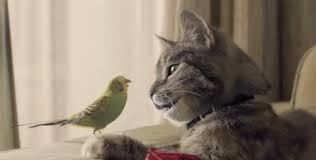
\includegraphics[width=0.5\textwidth]{images/sample_multi_label.PNG}
  \caption{Sample Multi-Label Image}\label{sample_multi_label}
\end{figure}


\begin{figure}
  \centering
  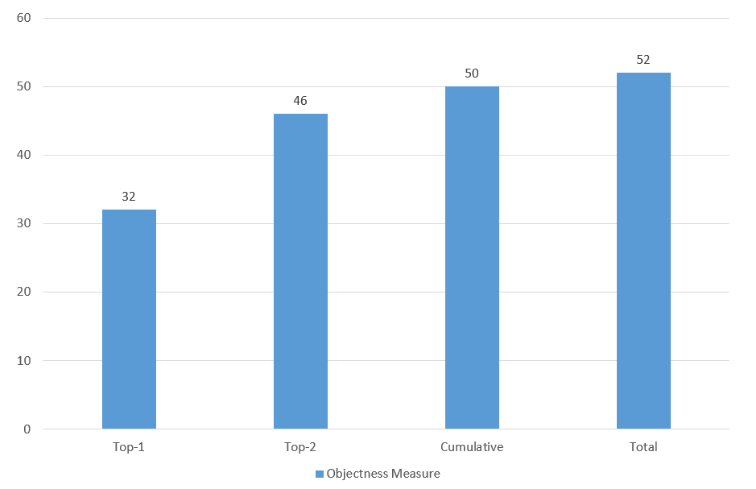
\includegraphics[width=0.5\textwidth]{images/Capture3.PNG}
  \caption{Result for multi-label images for Objectness Measures}\label{finobj}
\end{figure}


\begin{figure}
  \centering
  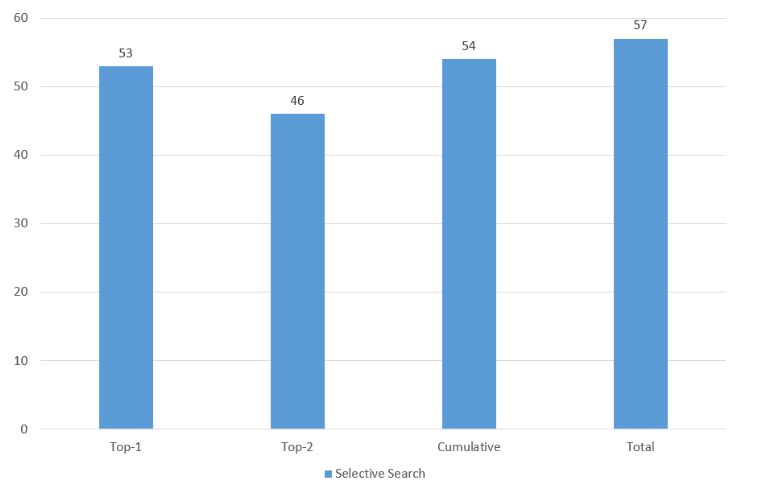
\includegraphics[width=0.5\textwidth]{images/Capture4.PNG}
  \caption {Result for multi-label images for Selective Search}\label{finsel}
\end{figure}

\section{Discussion}

The main problem of tagging multi-label images are the training time required. If Convolutional Neural Network is used for tagging multiple labels, then there is a chance that the networks will be very complex. This will require a lot of time to train. Also, if it takes a lot of time to train, then tweaking the network and exploring promising functionalities will require a lot of time. But our Convolutional Neural Network can only tag Single Label images, then we use this network to tag the segmented images provided by Objectness Measures and Selective Search approach. The Convolutional Neural Network we provided is faster to train, so tweaking the network will provide quick result. We got about 57\% accuracy using the Selective Search approach shown in \ref{finsel}. So, we can expect that if we increase the capability of our network, this accuracy will be much higher.



\section{Future Work}
The strength of our multi-label image classification architecture depends on convolutional neural network classifier and the method for segmenting images.So, be refining out convolutional neural network to include more labels by training CIFAR-100 and using better methods to segment the image, we can improve the performance of the network.As the image segmentation techniques give duplicate segmented images, so to sort out all the unique segmented images can be a nice challenge to achieve.







\section{Conclusion}
We have presented an easy and simple approach to classify multi-label images using a trained CNN classifier with objectness measure and selective search of an image. It gave us the result in quick time. Our training time for CNN network is fast. Segmenting the images is also fast. Our technique is a stepping stone to this approach. It is giving a good threshold result. In the future, this model can be enhanced and cope with larger dataset. So it will be interesting to see how advancement is made in this approach.
% if have a single appendix:
%\appendix[Proof of the Zonklar Equations]
% or
%\appendix  % for no appendix heading
% do not use \section anymore after \appendix, only \section*
% is possibly needed

% use appendices with more than one appendix
% then use \section to start each appendix
% you must declare a \section before using any
% \subsection or using \label (\appendices by itself
% starts a section numbered zero.)
%


%\appendices
%\section{Proof of the First Zonklar Equation}
%\blindtext

% use section* for acknowledgement
%\section*{Acknowledgment}
%
%
%The authors would like to thank...


% Can use something like this to put references on a page
% by themselves when using endfloat and the captionsoff option.
\ifCLASSOPTIONcaptionsoff
  \newpage
\fi


% trigger a \newpage just before the given reference
% number - used to balance the columns on the last page
% adjust value as needed - may need to be readjusted if
% the document is modified later
%\IEEEtriggeratref{8}
% The "triggered" command can be changed if desired:
%\IEEEtriggercmd{\enlargethispage{-5in}}

% references section

% can use a bibliography generated by BibTeX as a .bbl file
% BibTeX documentation can be easily obtained at:
% http://www.ctan.org/tex-archive/biblio/bibtex/contrib/doc/
% The IEEEtran BibTeX style support page is at:
% http://www.michaelshell.org/tex/ieeetran/bibtex/
%\bibliographystyle{IEEEtran}
% argument is your BibTeX string definitions and bibliography database(s)
%\bibliography{IEEEabrv,../bib/paper}
%
% <OR> manually copy in the resultant .bbl file
% set second argument of \begin to the number of references
% (used to reserve space for the reference number labels box)
\begin{thebibliography}{150}
 \bibitem {1} Alexe, B., Deselares, T. and Ferrari.
 Measuring the objectness of image windows. V. PAMI 2012.
 
 \bibitem {2} R. R. Uijlings, Koen E. A. van de Sande, Theo Gevers, Arnold W. M. Smeulders. 
Selective Search for Object Recognition, Jasper  International Journal of Computer Vision, Volume 104 (2), page 154-171, 2013.
 

\bibitem {3} A. Krizhevsky, I. Sutskever, and G. Hinton. Imagenet classification with deep convolutional neural networks. In Neural
Information Processing Systems, pages 1106–1114, 2012.

\bibitem {4} Dataset of CIFAR-10 https://www.cs.toronto.edu/~kriz/cifar.html.


\bibitem {5} Y. Gong, Y. Jia, T. K. leung, A. Toshev, and S. Ioffe. deep
convolutional ranking for multi label image annotation. In
International Conference on Learning Representations, 2014.

\bibitem{6} Sergey Ioffe, Christian Szegedy.
 Batch Normalization: Accelerating Deep Network Training by Reducing
Internal Covariate Shift.

\bibitem{7} P. F. Felzenszwalb and D. P. Huttenlocher. Efficient Graph Based Image Segmentation. IJCV, 59:167–181, 2004.


%\bibitem{IEEEhowto:kopka}
%%H.~Kopka and P.~W. Daly, \emph{A Guide to \LaTeX}, 3rd~ed.\hskip 1em plus
%%  0.5em minus 0.4em\relax Harlow, England: Addison-Wesley, 1999.
% Alexe, B., Deselares, T. and Ferrari.
% Measuring the objectness of image windows. V. PAMI 2012.
\end{thebibliography}

% biography section
% 
% If you have an EPS/PDF photo (graphicx package needed) extra braces are
% needed around the contents of the optional argument to biography to prevent
% the LaTeX parser from getting confused when it sees the complicated
% \includegraphics command within an optional argument. (You could create
% your own custom macro containing the \includegraphics command to make things
% simpler here.)
%\begin{biography}[{\includegraphics[width=1in,height=1.25in,clip,keepaspectratio]{mshell}}]{Michael Shell}
% or if you just want to reserve a space for a photo:

%\begin{IEEEbiography}[{\includegraphics[width=1in,height=1.25in,clip,keepaspectratio]{picture}}]{John Doe}
%% \bibitem {1} Alexe, B., Deselares, T. and Ferrari.
 Measuring the objectness of image windows. V. PAMI 2012.
 
 \bibitem {2} R. R. Uijlings, Koen E. A. van de Sande, Theo Gevers, Arnold W. M. Smeulders. 
Selective Search for Object Recognition, Jasper  International Journal of Computer Vision, Volume 104 (2), page 154-171, 2013.
 

\bibitem {3} A. Krizhevsky, I. Sutskever, and G. Hinton. Imagenet classification with deep convolutional neural networks. In Neural
Information Processing Systems, pages 1106–1114, 2012.

\bibitem {4} Dataset of CIFAR-10 https://www.cs.toronto.edu/~kriz/cifar.html.


\bibitem {5} Y. Gong, Y. Jia, T. K. leung, A. Toshev, and S. Ioffe. deep
convolutional ranking for multi label image annotation. In
International Conference on Learning Representations, 2014.

\bibitem{6} Sergey Ioffe, Christian Szegedy.
 Batch Normalization: Accelerating Deep Network Training by Reducing
Internal Covariate Shift.

\bibitem{7} P. F. Felzenszwalb and D. P. Huttenlocher. Efficient Graph Based Image Segmentation. IJCV, 59:167–181, 2004.

% \bibitem {1} Alexe, B., Deselares, T. and Ferrari.
% Measuring the objectness of image windows. V. PAMI 2012.
%\end{IEEEbiography}

% You can push biographies down or up by placing
% a \vfill before or after them. The appropriate
% use of \vfill depends on what kind of text is
% on the last page and whether or not the columns
% are being equalized.

%\vfill

% Can be used to pull up biographies so that the bottom of the last one
% is flush with the other column.
%\enlargethispage{-5in}


% that's all folks
\end{document}


